
\subsection{Parámetros que elegimos}

INSERTAR PARAMETROS Y RAZONES.

\subsection{Comparación con el algoritmo exacto}

Algo interesante que podemos preguntarnos es cómo se comparan nuestros algoritmos con el algoritmo exacto.

Sin embargo, como vimos anteriormente, el algoritmo exacto es extremadamente lento, por lo que un experimento ``clásico'', en el que se generan casos al azar y se corren los algoritmos sobre ellos no es viable.

Por esta razón, decidimos elegir una familia de grafos para la cual conozcamos de antemano, por sus características, la solución exacta, sin necesidad de correr el algoritmo exacto. 

Esta familia es precisamente la familia que encontramos como ``contraejemplo'' en el ejercicio del algoritmo goloso. Era la familia que nos permitía demostrar que el algoritmo no es $\alpha$-aproximado para ningún $\alpha > 0$. 

Recordemos los grafos y analicemos sus propiedades.


\begin{tikzpicture}[shorten >=1pt,auto,node distance=1.9cm,
                    semithick]
  \tikzstyle{every state}=[fill=red,draw=none,text=white]

	\node[state]	(0)		 		  {$2$};
	\node[state]	(1) [right of=0]  {$4$};
	\node[state]	(2) [below of=0]  {$3$};
	\node[state]	(3) [left of=0] 	  {$0$};
	\node[state]	(4) [above of=0]	  {$1$};
	\node[state]	(5) [right of=1]	  {$5$};
	\node[state]	(6) [above of=5]  {$6$};
	\node[state]	(7) [right of=6]  {$7$};
	\node[state]	(8) [right of=5]  {$8$};
	\node[state, fill=blue]	(9) [right of=8]	  {$0$};
	\node[state, fill=blue]	(10) [above of=9]  {$1$};
	\node[state, fill=blue]	(11) [right of=9]  {$2$};
	\node[state, fill=blue]	(12) [right of=10]  {$3$};


	\path	
		(0) edge[]				node {} (1)
         	edge[]				node {} (2)
         	edge[]				node {} (4)
         	edge[]				node {} (3)
		(1) edge[]				node {} (5)
		(5) edge[]				node {} (6)
		    edge[]				node {} (7)
		    edge[]				node {} (8)
		(6) edge[]				node {} (7)
		    edge[]				node {} (8)
		(7) edge[]				node {} (8)
		(9) edge[]				node {} (10)
		    edge[]				node {} (11)
		    edge[]				node {} (12)
		(10) edge[]				node {} (11)
		    edge[]				node {} (12)
		(11) edge[]				node {} (12);

\end{tikzpicture}

En nuestro caso utilizaremos una pequeña variación de este grafo (la única diferencia es que la arista que une a la estrella con el completo no sale de un brazo, si no de el centro de la estrella).

Como vimos anteriormente, el algoritmo goloso devuelve una solución muy mala siempre, dado que mapea al grafo completo azul con el grafo estrella rojo. 

Otra cosa que puede observarse es que, por como son nuestras heurísticas de búsqueda local, esa solución (la del goloso) es un mínimo local para todas estas soluciones. Esto puede chequearse muy fácilmente viendo la forma de los grafos y las soluciones (cualquier vecino a la solución del goloso es igual o peor que la solución del goloso).

Sin embargo, el tabú search viene a solucionar este problema, debido a la función de aspiración, que nos permite saltar a una solución aunque sea peor que la que tenemos, si todas lo son.

Enunciadas nuestras hipótesis sobre la experimentación, veamos los resultados.

\begin{figure}[H]
 \centering
	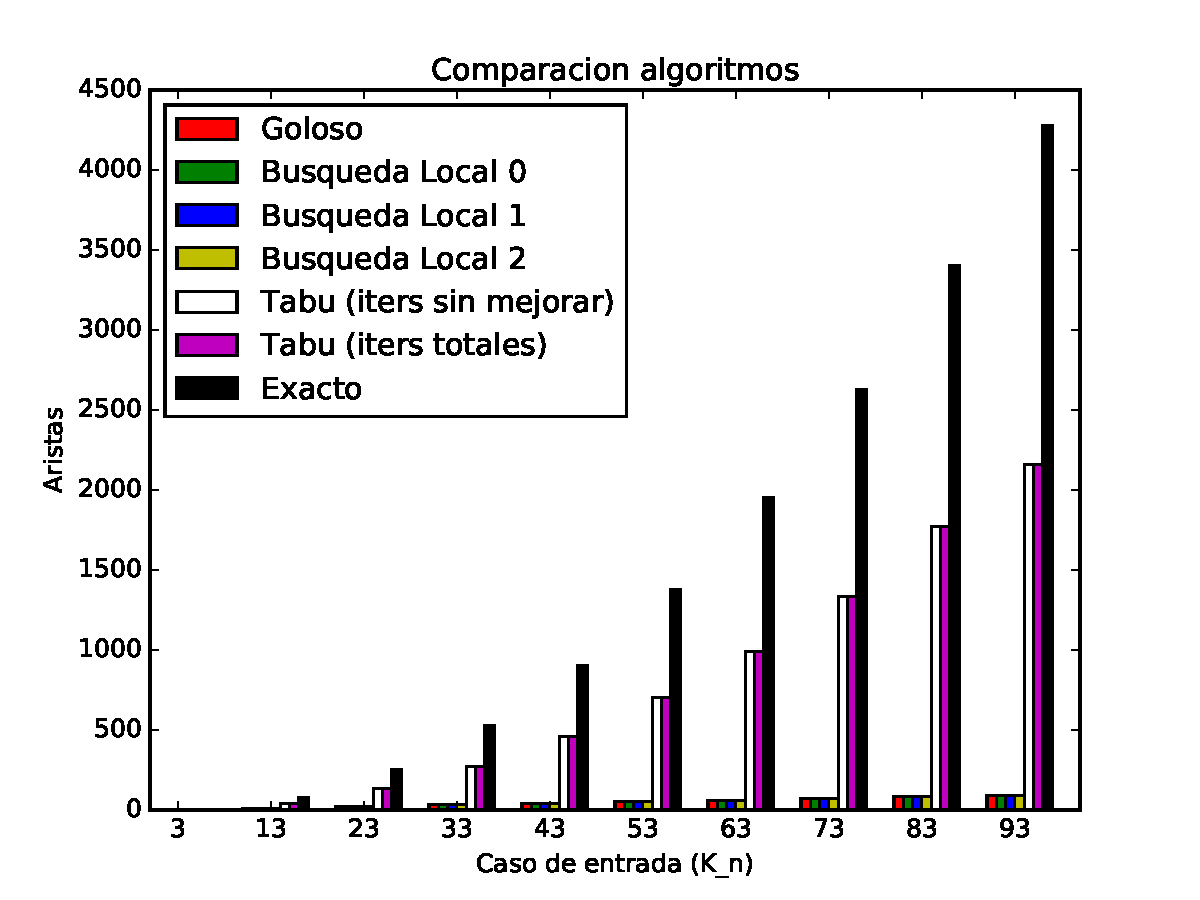
\includegraphics[width=0.9\textwidth]{graficos/problema_7/exacto0.pdf}
	\caption{}
	\label{fig:problema7-exacto0}
\end{figure}


Puede verse que sucede lo que esperabamos. Es decir, la solución del algoritmo goloso es muy mala, y la de las búsquedas locales no lo mejora.

Sin embargo, el tabú search permite mejorar mucho las soluciones. De todos modos, al igual que antes, no se observan diferencias notorias entre los dos criterios de parada del algoritmo: el secreto del éxito reside en las buenas vecidades que elegimos.



